\def\beginanswers{\iffalse}
%%\def\beginanswers{\iftrue}

\documentclass[10pt]{article}
\usepackage{amsmath,amsfonts,amsthm,amssymb}
\usepackage{graphicx}
\usepackage{enumerate}
\usepackage{upquote,textcomp}
\usepackage{listings}
\usepackage{color}

\definecolor{mygreen}{rgb}{0,0.6,0}
\definecolor{mygray}{rgb}{0.5,0.5,0.5}
\definecolor{mymauve}{rgb}{0.58,0,0.82}


\lstset{frame=tb,
  language=,
  aboveskip=3mm,
  belowskip=3mm,
  showstringspaces=false,
  columns=flexible,
  keepspaces=true,
  basicstyle={\small\ttfamily},
  numbers=none,
  numberstyle=\tiny\color{black},
  keywordstyle=\color{black},
  commentstyle=\color{black},
  stringstyle=\color{black},
  breaklines=true,
  breakatwhitespace=true,
  tabsize=3
}

\lstset{frame=tb,
  language=Python,
  aboveskip=3mm,
  belowskip=3mm,
  showstringspaces=false,
  columns=flexible,
  basicstyle={\small\ttfamily},
  numbers=none,
  numberstyle=\tiny\color{mygray},
  keywordstyle=\color{blue},
  commentstyle=\color{mygreen},
  stringstyle=\color{mymauve},
  breaklines=true,
  breakatwhitespace=true,
  tabsize=3
}


\newcommand{\vect}[1]{{\bf #1}}                 %for bold chars
\newcommand{\vecg}[1]{\mbox{\boldmath $ #1 $}}  %for bold greek chars
\newcommand{\matx}[1]{{\bf #1}}

\setlength{\parindent}{0in}
\setlength{\parskip}{1em}
\setlength{\textheight}{9.5in}
\setlength{\textwidth}{7in}
\setlength{\headsep}{0in}        % distance from top of page to address
\setlength{\topmargin}{-0.5in}
\setlength{\oddsidemargin}{-0.5in}
\setlength{\evensidemargin}{-0.5in}


\begin{document}
\thispagestyle{empty}

\vspace*{0.5in}

\begin{center}
\Large
\textbf{Open Source Software --- CSCI-4470 --- Spring 2021} \\
\textbf{Test 2} \\
\textbf{April 20, 2021}
\end{center}


%%%%%%%%%%%%%%%%%%%%%%%%%%%%%%%%%%%%%%%%%%%%%%%%%%%%%%%%%%%%%%%%%%%%%%%%
%%%%%%%%%%%%%%%%%%%%%%%%%%%%%%%%%%%%%%%%%%%%%%%%%%%%%%%%%%%%%%%%%%%%%%%%
\beginanswers
\begin{center}
\Large
\textbf{SOLUTIONS}
\end{center}

%%%%%%%%%%%%%%%%%%%%%%%%%%%%%%%%%%%%%%%%%%%%%%%%%%%%%%%%%%%%%%%%%%%%%%%%
\else
%%%%%%%%%%%%%%%%%%%%%%%%%%%%%%%%%%%%%%%%%%%%%%%%%%%%%%%%%%%%%%%%%%%%%%%%


\begin{center}

\textbf{\Large Name:} \underline {\hspace{2.0in}} \\

\bigskip
\bigskip

\centerline{
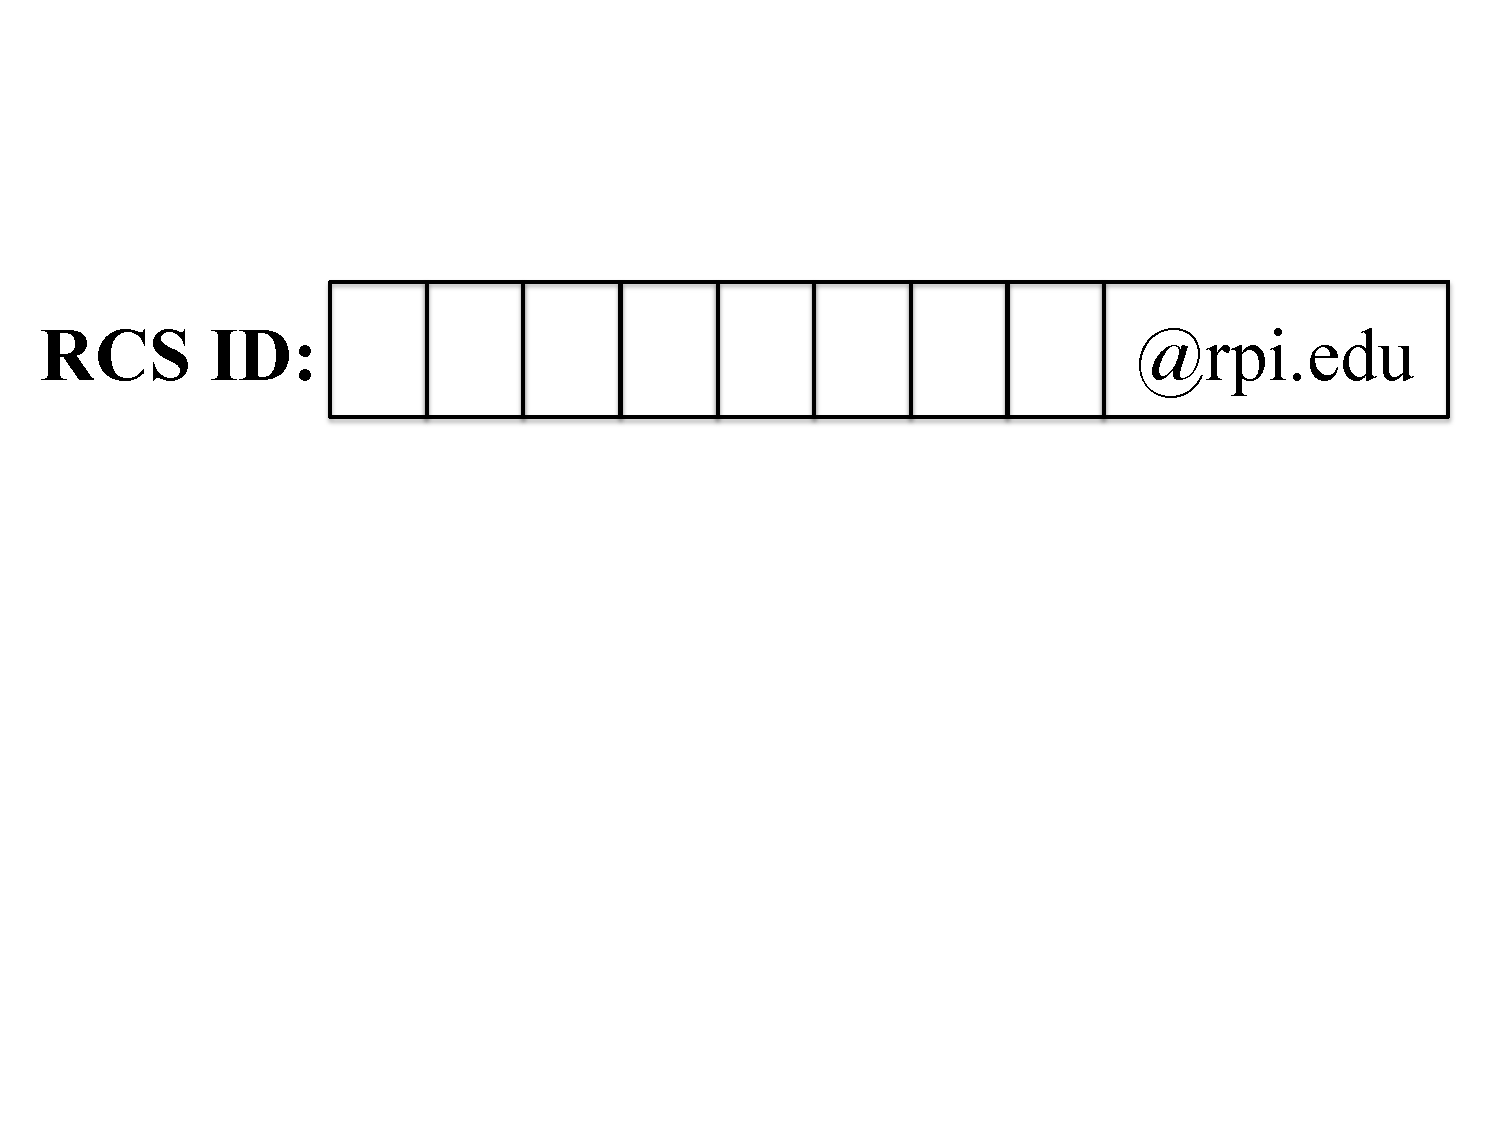
\includegraphics[height=0.5in]{boxes}
}

%%  \begin{tabular}{|p{0.1in}|p{0.1in}|p{0.1in}|p{0.1in}|p{0.1in}|p{0.1in}|p{0.1in}|p{0.1in}|l|}
%%    \hline \\
%%   & & & & & & & & \textbf{\large @rpi.edu} \\
%%  \hline
%%  \end{tabular} 
%%  
%%  \end{tabular}

\bigskip

\textbf{\Large RIN\#:} \underline {\hspace{1.5in}}  

\vspace*{0.4in}
{\large\bf Honor pledge: On my honor I have neither given
nor received aid on this exam.}

\vspace*{0.1in}
{\large\bf Please sign here to indicate that you agree with the honor pledge: \underline {\hspace{1.5in}}}
\end{center}

\vspace*{.45in} 

{\large\bf Instructions:}
\begin{itemize}
%%\item You have 90 minutes to complete this test.
\item Clearly print your name, RCS ID (in all caps.) and your RIN at the top of your exam.
\item This test is open book, open notes and open computer. You \textbf{may not} use the internet. Please turn off your wifi.
\item There are \textbf{6 questions} on this test worth a total of
  \textbf{100 points}.
\end{itemize}

\centering{\begin{tabular}{|c|c|r|}
	\hline
	Question & Score & Possible \\ \hline
	1 &  & 20 \\ \hline
	2 &  & 20 \\ \hline
	3 &  & 20 \\ \hline
	4 &  & 20 \\ \hline
	5 &  & 20 \\ \hline
	Total &  & 100 \\ \hline
\end{tabular}}

\newpage

%% ^\d?[\( ]?(\d{3})[- \)]*\d{3}[- \)]*\d{4}

%%%%%%%%%%%%%%%%%%%%%%%%%%%%%%%%%%%%%%%%%%%%%%%%%%%%%%%%%%%%%%%%%%%%%%%%
\fi
%%%%%%%%%%%%%%%%%%%%%%%%%%%%%%%%%%%%%%%%%%%%%%%%%%%%%%%%%%%%%%%%%%%%%%%%

\begin{enumerate}
	%% Spring 2021
	\item (20 points) The code below is extracted from the \textbf{Angry Birds} example we did 
		in class. Refer to it to answer the questions below.


		\lstinputlisting{code/Scientific/main.py}

		\newpage

		\beginanswers
		\begin{enumerate}

			\newpage

			\item (2 of 20 points) Which python package encapsulates the game play?

				\bigskip
				pygame
				\bigskip

			\item (2 of 20 points) Which python module ecapsulates the game physics?

				\bigskip
				pymunk
				\bigskip

			\item (4 of 20 points) Assume you want to add a 
				headwind blowing from right to left across the 
				screen. The force due to the headwind is one 
				tenth $\frac{1}{10}$ of the force of gravity in 
				the simulation. Write a short code snippet to 
				start the headwind and reset the gravity to Earth 
				normal, as currently defined in the simulation, 
				when the \verb|'h'| key is pressed. (Headwinds 
				don't occur in space.) Indicate where your code 
				should be inserted in the snippet provided. (Use 
				the provided line numbers.)

				\bigskip
				Insert the following ater line 40:
				\begin{lstlisting}
               			elif event.type == pygame.KEYDOWN and event.key == pygame.K_n:
                   			space.gravity = (-70.0, -700.0)
                   			level.bool_space = False
				\end{lstlisting}
				\bigskip
			
			\item (2 of 20 points) What would you change in your code if there was a tailwind 
				instead (blowing 
				from left to right.)

				\bigskip
				\begin{lstlisting}
               			elif event.type == pygame.KEYDOWN and event.key == pygame.K_n:
                   			space.gravity = (70.0, -700.0)
                   			level.bool_space = False
				\end{lstlisting}
				\bigskip

			\item (3 of 20 points) Which \textbf{pymunk} variable represents 
				the \textit{toggleable} \verb|wall| at 
				the right end of the laying field?

				\bigskip
                   		static\_lines1
				\bigskip

			\item (3 of 20 points) Which \textbf{pymunk} variable represents the \verb|floor| at 
				the bottom of the laying field?

				\bigskip
                   		static\_lines
				\bigskip


			\item (2 of 20 points) Which python module manages the frames per second?

				\bigskip
				pygame
				\bigskip

			\item (2 of 20 points) Which python module manages the collisions by invoking the 
				collision handlers?

				\bigskip
				pymunk
				\bigskip
                \end{enumerate}
		\else
		\begin{enumerate}
			\item (2 of 20 points) Which python package encapsulates the game play?
				\bigskip
				\bigskip
				\bigskip
				\bigskip
				\bigskip
				\bigskip
				\bigskip
				\bigskip
				\bigskip
				\bigskip

			\item (2 of 20 points) Which python module ecapsulates the game physics?
				\bigskip
				\bigskip
				\bigskip
				\bigskip
				\bigskip
				\bigskip
				\bigskip
				\bigskip
				\bigskip
				\bigskip

			\item (4 of 20 points) Assume you want to add a headwind blowing from right to left across the 
				screen. The force due to the headwind is one tenth $\frac{1}{10}$ of the 
				force of gravity in the simulation. Write a short code snippet to start the
				headwind when the \verb|'h'| and reset the gravity to Earth normal gravity
				as used in the simulation (headwinds don't occur in space).
				Indicate where your code should be inserted in the snippet provided. (Use the
				provided line numbers)
				\bigskip
				\bigskip
				\bigskip
				\bigskip
				\bigskip
				\bigskip
				\bigskip
				\bigskip
				\bigskip
				\bigskip
			
			\item (2 of 20 points) What would you change in your code if there was a tailwind instead (blowing 
				from left to right.)
				\bigskip
				\bigskip
				\bigskip
				\bigskip
				\bigskip
				\bigskip
				\bigskip
				\bigskip
				\bigskip
				\bigskip

			\item (3 of 20 points) Which \textbf{pymunk} variable represents the \textit{toggleable} \verb|wall| at 
				the right end of the laying field?
				\bigskip
				\bigskip
				\bigskip
				\bigskip
				\bigskip
				\bigskip
				\bigskip
				\bigskip
				\bigskip
				\bigskip

			\item (3 of 20 points) Which \textbf{pymunk} variable represents the \verb|floor| at 
				the bottom of the laying field?
				\bigskip
				\bigskip
				\bigskip
				\bigskip
				\bigskip
				\bigskip
				\bigskip
				\bigskip
				\bigskip
				\bigskip

			\item (2 of 20 points) Which python module manages the frames per second?
				\bigskip
				\bigskip
				\bigskip
				\bigskip
				\bigskip
				\bigskip
				\bigskip
				\bigskip
				\bigskip
				\bigskip

			\item (2 of 20 points) Which python module manages the collisions by invoking the 
				collision handlers?
				\bigskip
				\bigskip
				\bigskip
				\bigskip
				\bigskip
				\bigskip
				\bigskip
				\bigskip
				\bigskip
				\bigskip
                \end{enumerate}
		\fi

\newpage

    \item Assume you have 2 files of data. On each line of the first file is an \textbf{identifier} and a 
	    single \textbf{name} field. On each 
	    line of the second file is an \textbf{identifier} and a single favorite \textbf{drink} field. 

	    Example files are shown below:

	    \textbf{file1.txt}

	    \lstinputlisting{code/Database/file1.txt}

	    \textbf{file2.txt}

	    \lstinputlisting{code/Database/file2.txt}

	    Write a simple 
	    python program using \verb|'pymongo'| that reads both files and writes the data to a mongo 
	    collection. Data with the same \textbf{identifier} should be merged into the same document with
	    \textbf{identifier} as its unique document identifier. Use database \textbf{yankees} 
	    and collection name \textbf{menu}. After running your code on the sample
	    data, the following should be
	    stored in the database.

	    \lstinputlisting{code/Database/all.txt}

    \beginanswers
    	\lstinputlisting{code/Database/checkpoint4.py}
    \else
	\hspace*{-0.4in}\framebox(540,700){}
\fi

\newpage

\item (20 points) Refer to the \textbf{Github Action} template for \textbf{cmake} shown below while
	answering the following questions.
	
\lstinputlisting{code/Testing/cmake.yml}

\begin{enumerate}
	\item (4 of 20 points) What is the command that \textbf{builds} the test executables?
	
	\beginanswers
		\textbf{Answer:}

		\bigskip
		\verb|run: cmake --build . --config $BUILD_TYPE|
		\bigskip
	\else
	\bigskip
	\bigskip
	\bigskip
	\bigskip
	\bigskip
	\bigskip
	\bigskip
	\bigskip
	\bigskip
	\bigskip
	\fi

	\item (4 of 20 points) What platform and version do the tests run on?
	
	\beginanswers
		\textbf{Answer:}

		\bigskip
	ubuntu-latest
		\bigskip
	\else
	\bigskip
	\bigskip
	\bigskip
	\bigskip
	\bigskip
	\bigskip
	\bigskip
	\bigskip
	\bigskip
	\bigskip
	\fi

	\item (4 of 20 points) Assuming actions are set up correctly, what repository actions 
		cause this testing file
		to run?
	
	\beginanswers
		\textbf{Answer:}

		\bigskip
	When someone pushes or makes a pull request to the repository.
		\bigskip
	\else
	\bigskip
	\bigskip
	\bigskip
	\bigskip
	\bigskip
	\bigskip
	\bigskip
	\bigskip
	\bigskip
	\bigskip
	\fi

	\item (4 of 20 points) Modify the line that actually executes the tests so that it only
		runs tests 50 though 100.
	
	\beginanswers
		\textbf{Answer:}

		\bigskip
		\verb|run: ctest -C $BUILD_TYPE -I 50,100|
		\bigskip
	\else
	\bigskip
	\bigskip
	\bigskip
	\bigskip
	\bigskip
	\bigskip
	\bigskip
	\bigskip
	\bigskip
	\bigskip
	\fi

	\item (4 of 20 points) In our class notes we discussed errors, faults, and failures. Please discuss
		the meanings of the 3 terms and say which one testing is designed to discover.
	
	\beginanswers
		\textbf{Answer:}

		\bigskip
An error is made by an Engineer/Algorithm Designer/Implementor.
A fault is manifestation of that error in the code.
A failure is an incorrect output behavior that is caused by executing a fault.
Testing attempts to discover failures in software systems.
		\bigskip
	\else
	\bigskip
	\bigskip
	\bigskip
	\bigskip
	\bigskip
	\bigskip
	\bigskip
	\bigskip
	\bigskip
	\bigskip
	\bigskip
	\bigskip
	\bigskip
	\bigskip
	\bigskip
	\bigskip
	\bigskip
	\bigskip
	\bigskip
	\bigskip
	\bigskip
	\bigskip
	\fi

\end{enumerate}
	
\newpage


\item (20 points) I need a new Docker container to run my favorite programs. Write a \verb|Dockerfile| based off of the 
	latest \verb|python| release. I want it to have:


	\textbf{programs}: 
	\begin{itemize}
	        \item \verb|git|
	        \item \verb|emacs|
	\end{itemize}

	\textbf{python modules}:
	
	\begin{itemize}
		\item tensorflow
		\item matplotlib
	\end{itemize}

	\textbf{Finally, I need}:
	
	\begin{itemize}
		\item A directory \verb|/home/turner| to work in
		\item This should be the working directory
		\item The container should run \verb|bash| when it is started
	\end{itemize}

	\begin{enumerate} 
		\item (16/20 points) Write a \verb|Dockerfile| to provision the container described above.

\beginanswers
\lstinputlisting{code/Docker/Dockerfile}
\else
\hspace*{-0.4in}\framebox(540,460){}
\fi

\item (2/20 points) What command would be used to generate a container named \verb|favorites| from this Dockerfile? 
	You can assume you are in
	the same directory as the file.

\beginanswers
			\begin{lstlisting}
			docker build -t favorites .
			\end{lstlisting}
\else
\hspace*{-0.4in}\framebox(540,60){}
\fi

\item (2/20 points) What command would be used to run the container you just created so that it 
	comes up in interactive mode with a terminal prompt?

\beginanswers
			\begin{lstlisting}
			docker run -it favorites
			\end{lstlisting}
\else
\hspace*{-0.4in}\framebox(540,60){}
\fi

\end{enumerate}

\newpage

\item   (20 points) In class we used Tensorflow to find the $2$ coefficients $m$ and $b$ of the 
	linear equation $y = m*x + b$. For this question, 
	you will modify that code to find the three coefficients $a$, $b$, and $c$ of the quadratic equation 
	$y = a*x^2 + b*x + c$. A (slightly) modified version of the code from class is shown below along 
	with a plot of my solution to the quadratic equation $y = 0.5 * x^2 - 0.6 * x + 0.3$. The number of
	iterations for the plot was $2000$ and the learning rate was $0.4$. Note that I made
	two small changes to improve plotting. 

\begin{itemize}
	\item I changed the number of points in the test data from $100$ to $1000$.
	\item I changed the plot command to use red dots instead of blue lines.
\end{itemize}

	Modify the code below to solve quadratics. Make sure that you
	modify the code to generate the noisy data along with the code to calculate the solution.


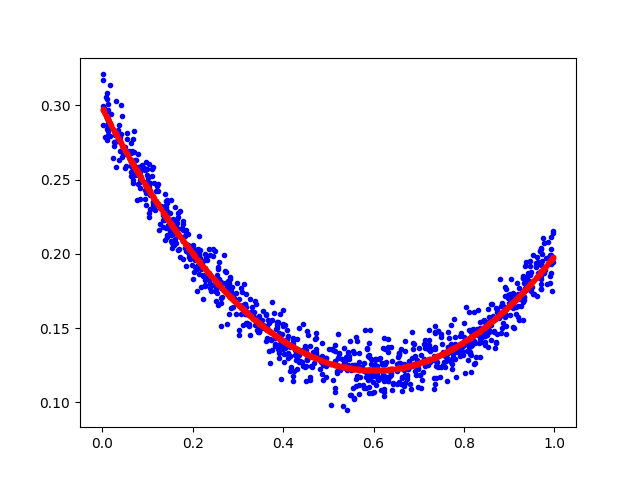
\includegraphics[width=0.6\linewidth]{images/quadratic.png}

\newpage

\lstinputlisting{code/Tensorflow/class.py}

\beginanswers
\textbf{Answer:}
\lstinputlisting{code/Tensorflow/quad.py}
\else
\hspace*{-0.4in}\framebox(540,700){}
\fi
\newpage

\end{enumerate}
\end{document}
